% Asset ID: FA22CentralLimitTheoremTikZ-001
% Used placeholder: [VISUAL PLACEHOLDER: FA22CentralLimitTheoremTikZ-001 | Source: CLT theorem + worked examples in transcript and slide PDF | Insert from tikz/FA22CentralLimitTheoremTikZ-001.tex | Purpose: Show how a sample-mean probability becomes a normal tail probability.]
\documentclass[tikz,border=8pt]{standalone}
\usepackage{amsmath}
\usetikzlibrary{arrows.meta}
\definecolor{Canvas}{HTML}{FAF9F6}\definecolor{Gold}{HTML}{C5A059}\definecolor{Rose}{HTML}{FBEFEF}\definecolor{Ink}{HTML}{2C2C2E}
\begin{document}
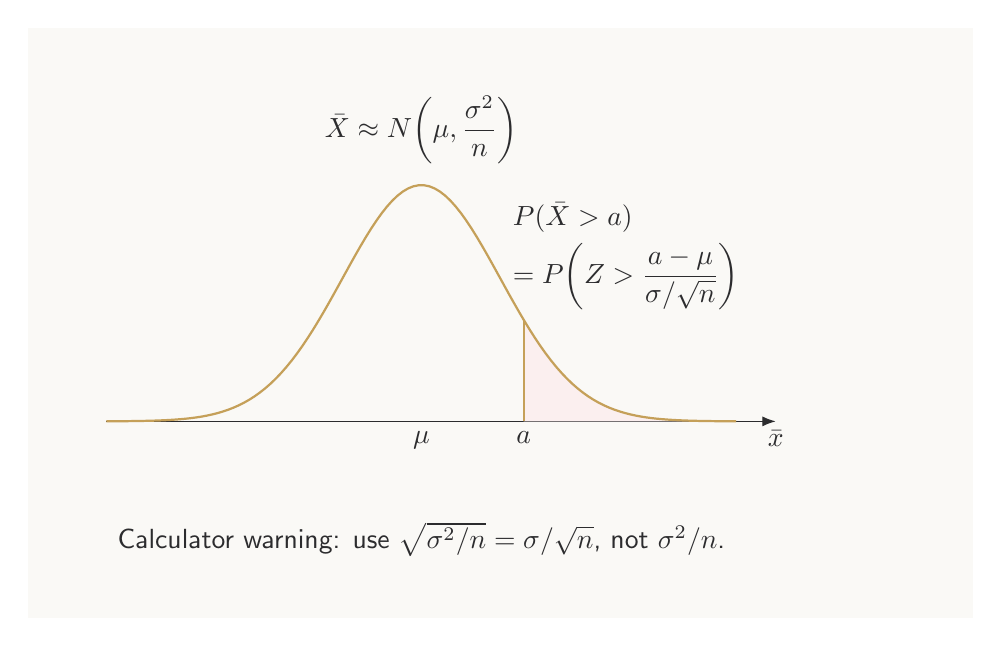
\begin{tikzpicture}[>=Latex,every node/.style={font=\sffamily,text=Ink}]
\fill[Canvas] (-5,-2.5) rectangle (7,5);
\draw[Ink,->] (-4,0)--(4.5,0) node[below]{$\bar x$};
\def\a{1.3}
\path[fill=Rose] (\a,0)--plot[domain=\a:4,samples=80](\x,{3*exp(-.5*\x*\x)})--(4,0)--cycle;
\draw[Gold,thick,samples=120,domain=-4:4] plot(\x,{3*exp(-.5*\x*\x)});
\draw[Gold,thick] (\a,0)--(\a,{3*exp(-.5*\a*\a)});
\node[below] at (0,0){$\mu$};\node[below] at (\a,0){$a$};
\node at (0,3.7){$\bar X\approx N\!\left(\mu,\dfrac{\sigma^2}{n}\right)$};
\node[align=left] at (2.6,2.1){$P(\bar X>a)$\\[3pt]$=P\!\left(Z>\dfrac{a-\mu}{\sigma/\sqrt n}\right)$};
\node at (0,-1.5){Calculator warning: use $\sqrt{\sigma^2/n}=\sigma/\sqrt n$, not $\sigma^2/n$.};
\end{tikzpicture}
\end{document}
